% !Mode:: "TeX:UTF-8"

\chapter{实验环境}

\section{Gym和Pyrobolearn}
Gym\cite{brockman2016openai}是一个由OpenAI团队开源的强化学习仿真环境,它已经成为了评价最先进的基线强化学习算法或机器人控制算法的标准环境。
Mujoco\cite{todorov2012mujoco}是一个著名的商业物理仿真引擎,它在强化学习和机器人学中得到广泛应用,并成为Gym中机器人相关的环境的默认仿真引擎。
在接下来的几章中,Gym将被用来验证算法正确性,或被用于更方便地与其他现有算法进行对比。

Gym提供一个Python语言的接口并且已经被包含在了Python包检索中。
Gym需要使用OpenGL的开源库GLFW来进行渲染。
它可以直接使用Python包管理器\emph{pip}进行安装。
在Gym中,有很多内置的环境,包含大量著名的和强化学习有关基本任务可用于验证强化学习算法,并提供了统一的接口。
例如,它包含一个经典的名为“推车杆”的控制任务,这个任务要求智能体通过水平地移动推车来平衡一个底部用自由活动的关节连接到推车上的杆。
一个正常的强化学习算法应当可以在较长时间内避免杆失去平衡并倒下。

Mujoco(Multi-Joint dynamics with Cotact)是一个致力于仿真复杂关节运动、碰撞和多物体接触的物理引擎。
它集成了粒子系统仿真、约束求解器、有限元积分器和凸优化器等等工具。
它使用ANSI C编写并有一个Python的API封装。
在Gym中,\emph{FetchReach-v1}环境需要使用Mujoco作为仿真器,因此在实验中Mujoco、OpenGL和Gym等工具都被安装在Ubuntu 20.04系统中,并设置了环境变量以保证正确的动态链接库\emph{libGL.so}和Mujoco的二进制分发被加载。

一个\emph{FetchReach-v1}环境的截图展示在图\ref{fetchreach-v1}中。
    \begin{figure}
        \centering
        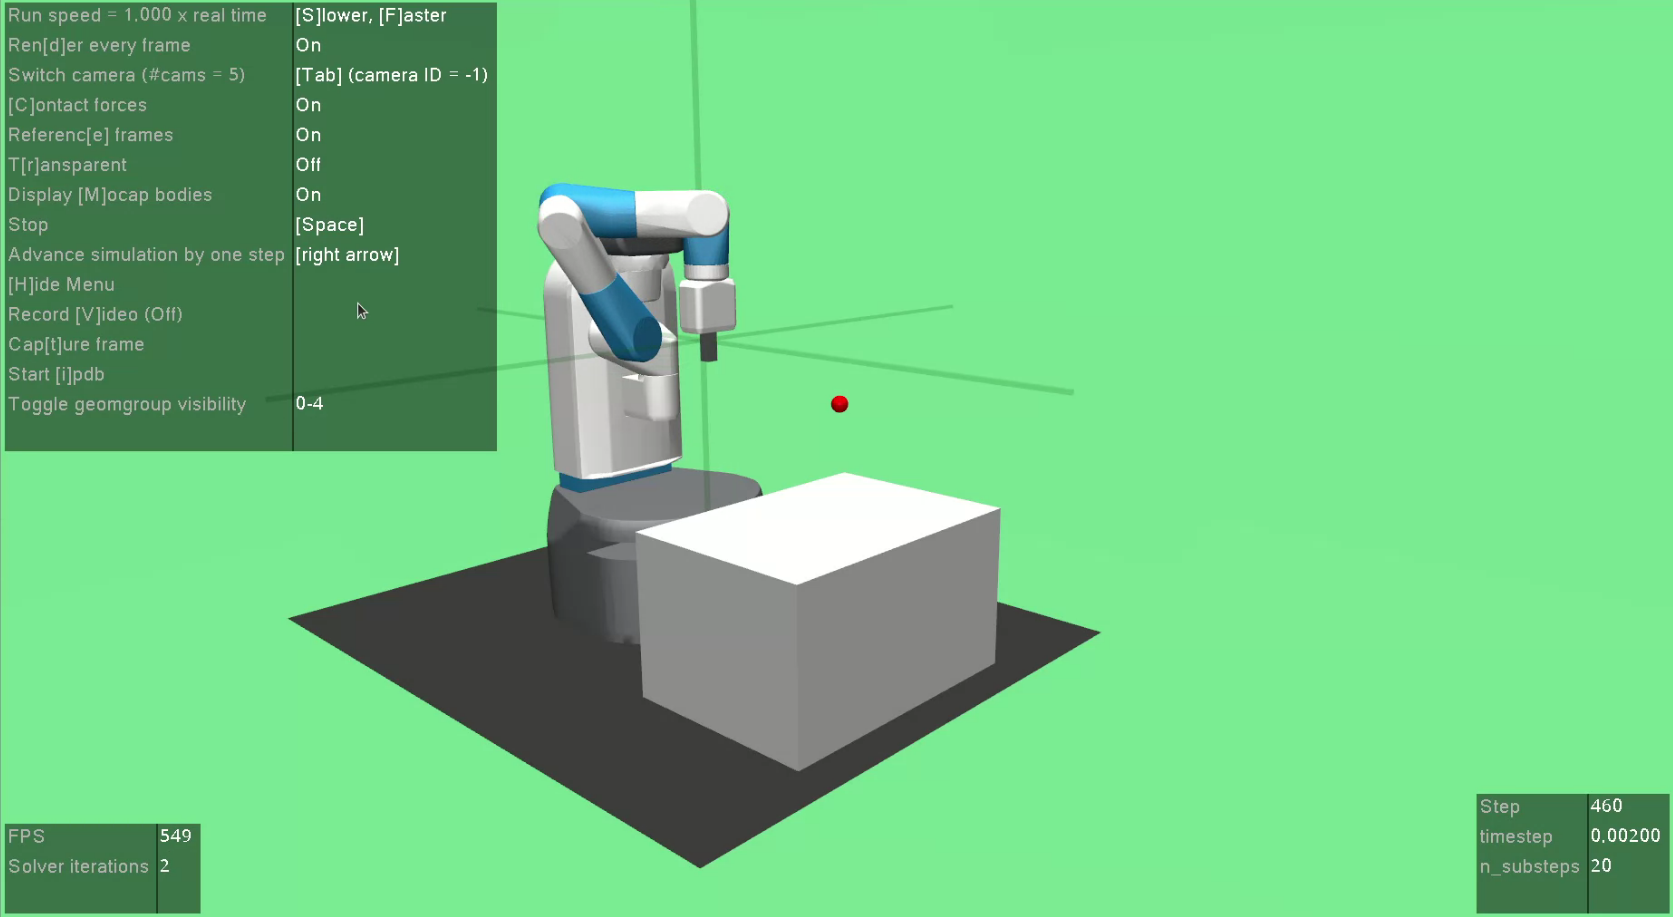
\includegraphics[width=0.8\textwidth]{fetchreach-v1.png}
        \caption{FetchReach-v1环境的截图}
        \label{fetchreach-v1}
    \end{figure}
其中有一个机械臂被放在一张桌子前。
在每个片段刚开始时,这个机械臂的状态都会被重置,而一个红点则会随机地出现在桌子上方的某处。
机械臂智能体需要在片段的限制时间内使自己的末端执行器到达这个红点附近来完成任务并获得奖励。
在片段的每一个时间步中,都会有观测值提供给此机械臂智能体。
观测值包括指示关节状态、末端执行器位置坐标信息作为已完成的目标,和红点的位置坐标信息作为期望目标。
指示关节状态的观测值$o\in \mathbb R^{10}$是一个10维的向量,而末端执行器的坐标$g^a \in \mathbb R^3$和红点的位置坐标$g^d\in\mathbb R^3$都是3维的向量。
因此提供给机械臂智能体的状态向量是一个16维的向量$s=(o, g^a, g^d)\in \mathbb R^{16}$。
如果末端执行器和红点之间的距离小于一个阈值,一个值为0.0的奖励会被提供给机械臂智能体,否则一个值为-1.0的奖励会被提供给它。
机械臂可以采取的动作是一个4维的取值在-1到1之间的向量,即$a\in[-1,1]^4$。

\section{Pyrobolearn和Pybullet}
虽然使用Gym和Mujoco的功能已经可以覆盖本课题的大部分实验,但是由于Mujoco是商业仿真软件,且可定制性不强,因此有必要使用开源的替代品,即Pyrobolearn和Pybullet,来设计本课题中的主体实验。

Pyrobolearn是一个专门设计来训练智能机器人的框架\cite{delhaisse2019pyrobolearn}。
它目前仍然在开发中,但是大部分实验中用到的功能已经足够稳定。
一些尚未在其中实现的功能也可以通过继承现有类来进行自定义。
与Gym相似,Pyrobolearn也有一个默认的物理引擎。
这个物理引擎叫做Pybullet\cite{coumans2016pybullet}。
它是一个C++编写的开源的物理引擎Bullet3在Python接口的封装,并可以提供本文中需要的所有仿真功能。它可以实时地检测碰撞,并可以精确地仿真多物理现象,这保证了它可以被用于本文需要的机器人和物体交互仿真的研究需求。
虽然Pyrobolearn也有一个使用Mujoco作为仿真器的接口,但是它对Mujoco的支持尚未稳定,因此本文的实验选择了使用Pybullet作为仿真器。

使用Pybullet作为仿真器,Pyrobolearn可以被用来仿真多种经典的机器人控制和强化学习问题。
实际使用中,一个物理世界对象包含了一些固定的物理量,例如重力方向和摩擦系数,并可以加载物体和机器人。
一个世界对象在构造过程中通常要提供一个仿真器,本文提供了Pybullet作为仿真器。
在世界对象构造完成后一个由仿真器生成的世界相机会被提供给世界对象作为一个属性。

在接下来的使用Pyrobolearn的实验中,全部都使用了\emph{Basic World}类型的世界对象,其中重力加速度向量为笛卡尔坐标系中的(0.0, 0.0, -9.81),横向摩擦系数为1.0,旋转摩擦系数为0.0,滚动摩擦系数为0.0,线性阻尼为0.04,角阻尼为0.04。

渲染后的世界相机下的\emph{Basic World}世界如图\ref{basicworld}所示。
    \begin{figure}
        \centering
        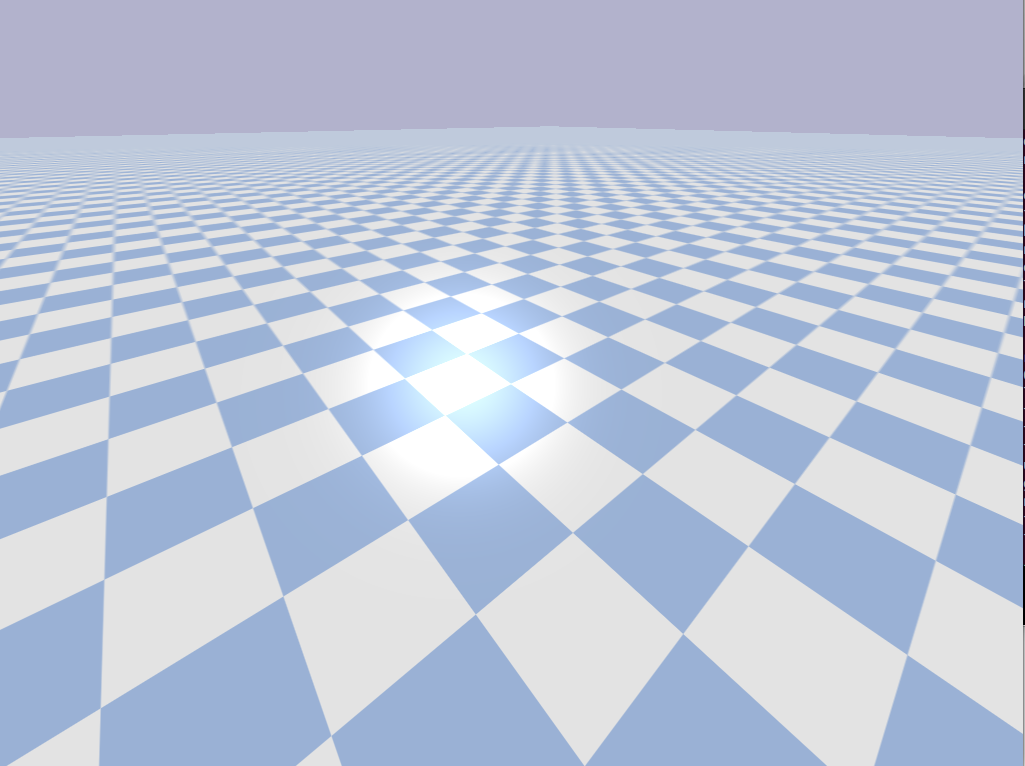
\includegraphics[width=0.3\textwidth]{basicworld.png}
        \caption{空白的\emph{Basic World}世界渲染结果}
        \label{basicworld}
    \end{figure}
默认情况下,没有物体和机器人被加载,只有地面和基本物理量被初始化。

两种不同的机械臂分别在初步实验和主体实验中使用。其中一个来自于Gym环境,另一个来自于Pyrobolearn框架。

在基于Mujoco的几个Gym环境中,一个和Fetch研究平台中的Fetch便携机械臂具有相同参数的机械臂被用作默认的唯一一个与环境交互的机器人\cite{Wise2016FetchF}。
Fetch便携机械臂有7个自由度。
在本文中使用到的\emph{FetchReach-v1}环境中,只有其中的4个被使用。
如第1节所述,\emph{FetchReach-v1}环境中的状态向量由Fetch机械臂的关节的位置信息、末端执行器的笛卡尔坐标和红点的笛卡尔坐标构成。

Pyrobolearn框架中的主体实验使用了一个叫做WAM的机械臂。
WAM机械臂可以配备手指终端执行器,它们一共有15个自由度,这意味着动作空间是非常高维的。
在\emph{Basic World}世界中加载的WAM机器人如图\ref{wam}所示。
    \begin{figure}
        \centering
        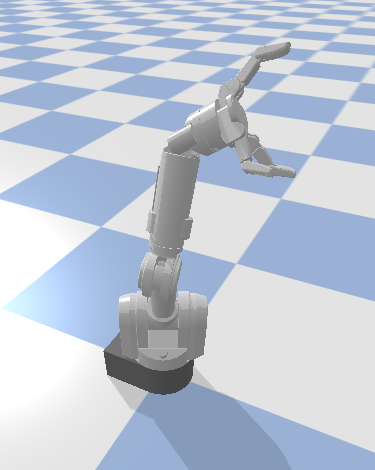
\includegraphics[height=0.3\textwidth]{wam.png}
        \caption{\emph{Basic World}中的WAM机器人渲染结果}
        \label{wam}
    \end{figure}

\section{实验框架}
本文中所有的实验都有可更改目标的状态,这意味着智能体可以获知当前已完成的目标和期望的目标。
假设期望的目标用一个3维的笛卡尔坐标表示,已完成的目标用机器人的末端执行器的笛卡尔坐标表示。
通常情况下,当这两个坐标间的距离小于一个阈值时,表示任务已经顺利完成。

形式化地,一个状态向量$s\in\mathcal S$是一个由3个向量构成向量,即$s=(o,g^a,g^d)$,其中$o$是观测到的环境中的物理量构成的向量,$g^a$是已完成的目标,$g^d$是期望的目标。
一个环境奖励函数$reward:\mathcal S\to \mathbb R$是由环境反馈决定的智能体在交互中可获得的奖励。

在实验中,因为目标可以方便地修改,所以可以使用事后经验重放算法,这也使得定义具有稀疏奖励的开放任务,并在其中使用多种方法训练高探索效率和泛化能力的智能体成为可能。

智能体与环境的交互在实验中被组织为分离的片段。
每个片段都有相同的最大时间步数$T$。
智能体应当在最大时间步数的限制$t\leq T$下完成一个特定的开放任务并获得较高的奖励。
对于\emph{FetchReach-v1}环境,最大的时间步数为50.
对于在Pyrobolearn框架下的主体实验中自定义的环境中,最大的时间步数为100或200.
智能体可以把在交互中获得的迁移信息$(s_t,a_t,r_t,s_{t+1})$保存在重放缓存中以便之后采样和训练。

对每个片段,最后一个时间步的下一个状态$s_{T+1}$不应被用于训练,因为当环境处理这个状态时这个片段已经结束,因此它不会导致未来的任何奖励。
为了防止在训练过程中使用这个状态,可以引入一个掩膜变量$m$,并与根据$s_{t+1}$计算得出的动作价值函数值相乘。
当$t<T$时,令$m=1$,当达到最后一个时间步,即$t=T$时,令$m=0$,并将$m$和迁移信息一同放入重放缓存中以便训练时与上述动作价值函数相乘。

在每个实验的片段开始时都引入了随机初始化。

对于\emph{FetchReach-v1}环境中的实验,在片段的第一个时间步之前,Fetch便携机械臂的关节位置被初始化为一个固定的起始位置,由红点表示的期望目标则随机地初始化为桌面上的一个位置。

在自定义的Pyrobolearn环境中,在片段开始之前,WAM机械臂上的关节位置被随机初始化,期望的目标也被随机地初始化在1米以内,其中目标的$z$坐标被初始化为0.5,$x,y$则从$[-1,1]$的均匀随机分布中采样。
与\emph{FetchReach-v1}环境中相比,自定义的环境中机械臂的初始状态是随机的,这会给此开放任务带来更多的复杂性。
有时候WAM机械臂的随机初始状态距离目标非常远,这会导致任务理论上不可能完成。

\section{系统设计}

Gym环境下的实验程序按照类图\ref{gymuml}所示的方式组织。
其中Module是Pytorch中的神经网络模块,μNet和QNet通过继承自动获得反向传播的方法backward。
$\mu$,Q1和Q2分别是演员网络,评论家网络1和评论家网络2;$\mu$\_tar,Q1\_tar和Q2\_tar分别是对应的靶网络。
每调用一次TD3对象的learn方法,都会进行一个时间步的仿真,时间步计数器cnt\_step和片断计数器cnt\_epi相当地进行自增运算,并把生成的迁移$(s_t,a_t,r_t,mask_t,s_{t+1})$存入重放缓冲memory中。
    \begin{figure}
        \centering
        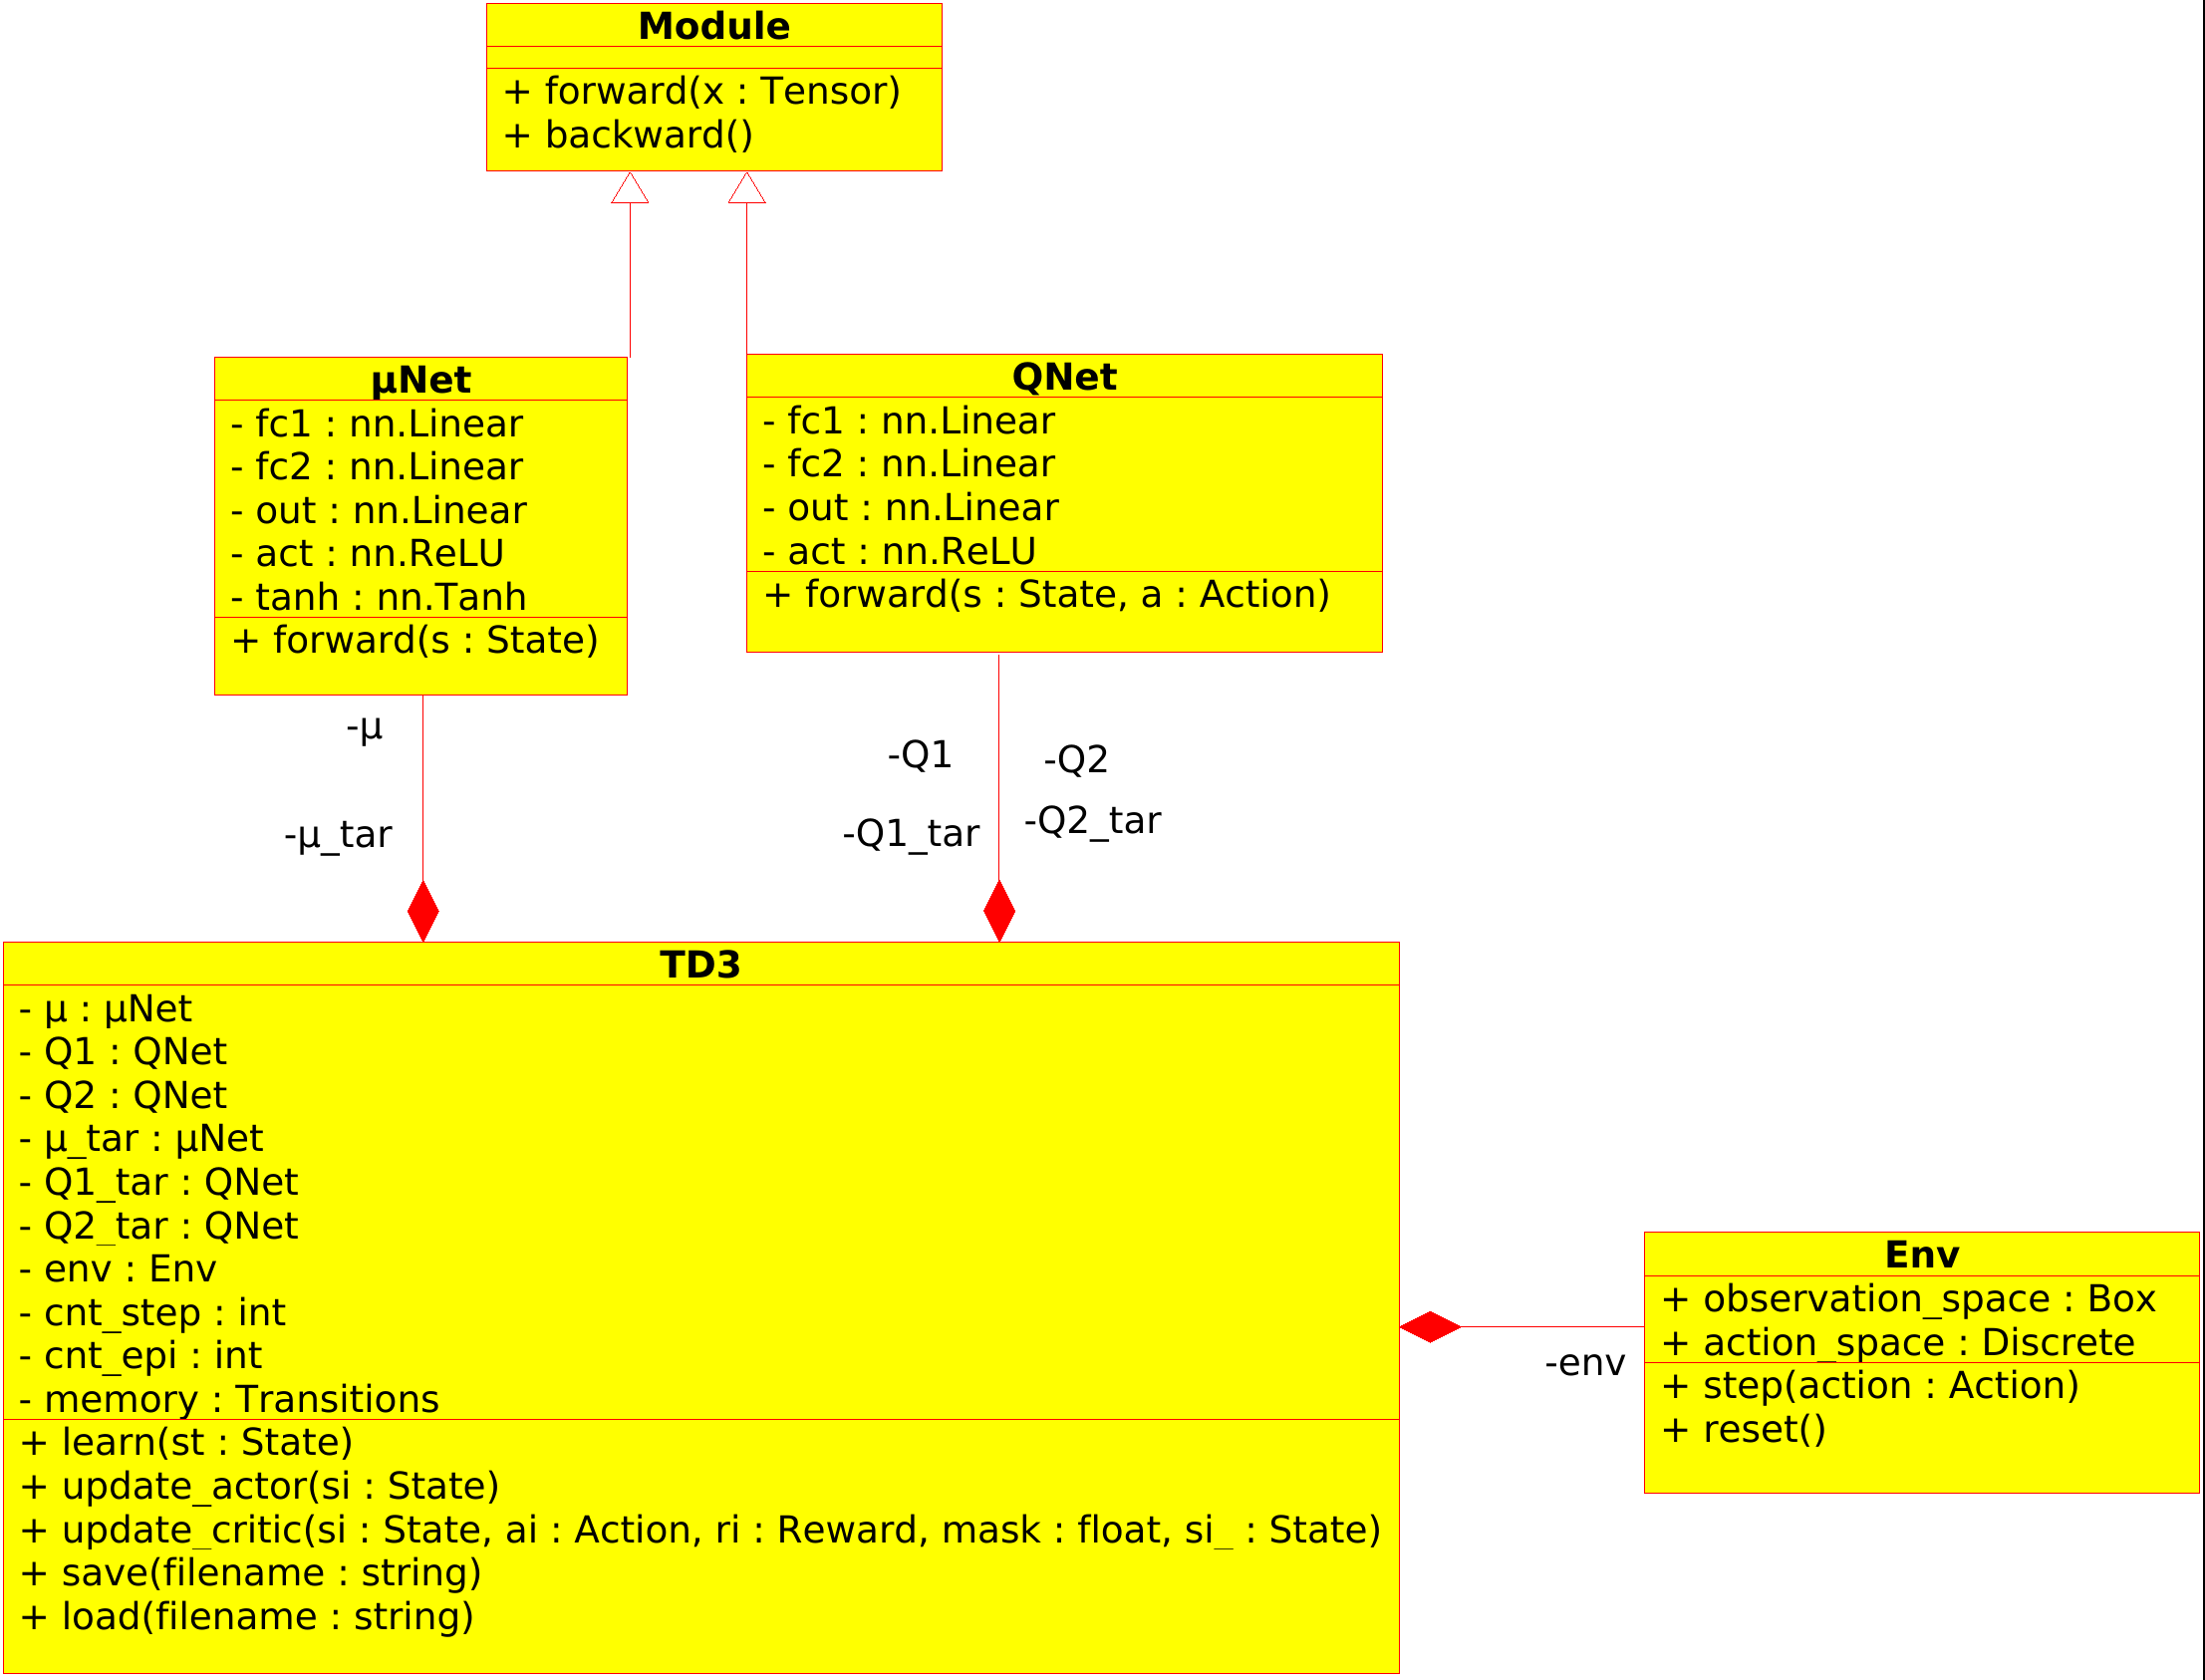
\includegraphics[height=0.6\textwidth]{gymuml.png}
        \caption{Gym实验程序类图}
        \label{gymuml}
    \end{figure}

% Local Variables:
% TeX-master: "../main"
% TeX-engine: xetex
% End:
